\chapter{Softwarequalität}
Für viele KundInnen ist Softwarearchitektur ein schwer einorden- und erklärbares Teilgebiet der Softwareentwicklung. Deswegen ist es schwierig, den/die KundIn für die Mithilfe an der Architekturerstellung und die daraus resultierenden Kosten zu gewinnen. Eine mögliche Lösung für dieses Problem ist es, die durch unzureichende Softwarequalität entstandenen Kosten, welche wiederum die Folge einer mangelhaften Architektur sind, den Kosten der Architekturerstellung gegenüber zu stellen.  \cite[S. 8-9]{softarch}


Eine gute Softwarearchitektur allein kann zwar nicht eine hohe Softwarequalität garantieren, ist jedoch ein wichtiger Faktor, ohne welchen keine hochqualitative Software erstellt werden kann. Softwarequalität und Softwarearchitektur stehen somit in einem engen Zusammenhang. \cite[S. 8-9]{softarch}

Was genau verbirgt sich jedoch hinter dem Begriff Softwarequalität? Der Begriff Qualität selbst ist sehr breit und schwer definierbar. Laut Garvin gibt es fünf verschiedene Herangehensweisen \cite[S. 25-29]{quality}:

\begin{itemize}
  \item Transzendentale Sicht
  \item Produktbasierte Sicht
  \item Userbasierte Sicht
  \item Herstellungsbasierte Sicht
  \item Wertbasierte Sicht
\end{itemize}

Die transzendentale Sicht beschreibt Qualität als sofort erkennbar, aber als nicht wirklich beschreibbar. Die produktbasierte Sicht ordnet die Qualität des Produktes dessen Bestandteilen zu. Bei der userbasierten Sicht geht es darum, die Anforderungen des/der NutzerInnen zu befriedigen: Die höchste Qualität eines Produktes wird daher erreicht, wenn der/die BenutzerIn alles vorfindet, was er/sie sich erwartet, nicht Mehr und nicht Weniger. Die herstellungsbasierte Sicht misst Qualität an der Erfüllung der Spezifikation und des Designs. Die wertbasierte Sicht schließlich definiert die Qualität durch das Preis-Leistungsverhältnis. \cite[S. 26]{quality}

Diese Sichten treffen mehr oder weniger auch für Softwarequalität zu \cite[S. 399]{pract}, sind aber noch zu grob formuliert, um konkrete Schritte bei der Erstellung des Systems und dessen Architektur zu setzen und konkrete Werte für die Überprüfung der Qualität fest zu legen. Eine genaue Auflistung der für Softwarequalität relevanten Faktoren, bzw. ein Modell, welches den Qualitätsprozess unterstützt, ist somit von Nöten.

\section{Softwarequalitätsmodelle}
ISO 9126 \cite{ISO_SQ} und dessen Nachfolger ISO 25010 \cite{ISO_SQ2} bieten ein Modell, um Softwarequalität zu beschreiben. ISO 25010, der Nachfolgestandard, erweitert die in ISO 9126 beschriebenen Hauptkategorien um Security und Compatibility. Auch die Kategorie Software Quality in Use erfährt eine Überarbeitung: Sie enthält nun die Kategorie Usability, welche vorher in den Hauptkriterien definiert war. Da es aber schwierig war, zitierbare Quellen zum neuen Standard zu finden - ISO 25010 hat \glqq in die Praxis wenig Einzug gehalten\grqq \ \cite[S. 60]{effektiv} - , die Neuerungen überschaubar und mehr eine Umorganisierung als Revolution darstellen, wird auf die Nutzung von ISO 25010 verzichtet und das Qualitätsmodell des Vorgängers, ISO 9216, verwendet.

ISO 9126 definiert folgende Qualitätskategorien:

\begin{itemize}
  \item \glqq Functionality\grqq
  \item \glqq Reliability\grqq
  \item \glqq Usability\grqq
  \item \glqq Efficiency\grqq
  \item \glqq Maintainability\grqq
  \item \glqq Portability\grqq
\end{itemize}


Die beschriebenen Kategorien können laut dem International Requirements Engineering Board, kurz IREB, wiederum in folgende Überkategorien eingeteilt werden: funktionale Anforderungen und nicht funktionale Anforderungen (Abbildung \ref{fig:iso9126}).

\begin{figure}[H]
    \centering
    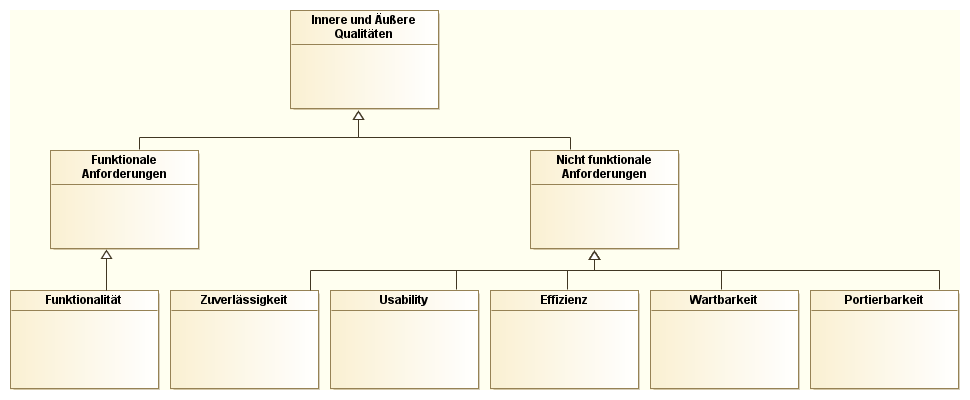
\includegraphics[scale=0.48]{img/iso9126.png}
    \caption{Die Qualitätskategorien des ISO 9126 Standards unterteilt in funktionale und nicht funktionale Anforderungen}
    \label{fig:iso9126}
\end{figure}


\section{Funktionale Anforderungen}
Funktionale Anforderungen beschreiben die Funktionalität des Systems, welche die Geschäftsprozesse des/der KundIn umsetzen und das System für ihn/sie somit wertvoll machen \cite[S. 79]{reqanalysis}. Sie werden vom/von der KundIn meist in der Form von Usecases beschrieben \cite[S. 78]{reqanalysis}

IREB ordnet die Functionality Kategorie von ISO 9126 den funktionalen Anforderungen zu\cite[S. 9]{ireb}, welche sich in folgende Unterkategorien aufspaltet:

\begin{itemize}
  \item \glqq Suitability\grqq
  \item \glqq Accuracy\grqq
  \item \glqq Interoperability\grqq
  \item \glqq Security\grqq
  \item \glqq Functional compliance\grqq
\end{itemize}

Suitability beschreibt das Vorhandensein von Funktionen, welche die vom/von der NutzerIn geforderten Funktionalitäten bereitstellen. Accuracy behandelt die geforderte Genauigkeit der implementierten Funktionen, Interoperability wiederum die Interaktionsmöglichkeiten des Systems mit anderen Systemen. Security beschreibt die implementierten Kontroll- und Sicherheitsmechanismen, mit welchen das System die Daten vor unerlaubtem Zugriff schützt. Der letzte Punkt, Functional Compliance, beschreibt die Standard- und Gesetzeskonformität des Softwareprodukts. \cite[S. 8]{ISO_SQ}

\section{Nicht funktionale Anforderungen}
Nicht funktionalen Anforderungen \glqq verkörpern Erwartungen und Notwendigkeiten, die von Interessensvertretern (Auftraggeber, Benutzer, Architekt, Entwickler, etc.) neben den funktionalen Anforderungen als wichtig erachtet werden und über die reine gewünschte Funktionalität hinausgehen\grqq \cite[S. 108]{softarch}. Sie definieren nicht das Was sondern das Wie \cite[S. 80]{reqanalysis}.

Der Fokus liegt meist auf der Funktionalität eines Systems; es ist schließlich der Hauptgrund für die Erstellung des Systems und der/die KundIn hat eine genaue Vorstellung, was das System genau können muss. Die Qualität des Systems ist meist eine implizite Anforderung, welche im Anforderungsprozess besonders beachtet werden muss, aber trotzdem essentiell für den Erfolg des Systems ist. \cite[S. 109]{softarch}

Dies lässt an folgendem Beispiel demonstrieren: Ein/Eine KundIn beauftragt eine Firma, einen Webshop zu erstellen, auf welchem er/sie seine/ihre Produkte verkaufen will. Die Funktionalität des Webshops wird wie beschrieben implementiert, aber das Endprodukt ist so langsam, dass ein Großteil der KundInnen den Bestellvorgang abbricht. Der Hauptfunktion des Systems, nämlich Produkte verkaufen, ist somit zwar prinzipiell möglich, aber für den/die KundIn im Vergleich zur investierten Summe unrentabel.

Nicht funktionale Anforderungen sind nicht nur oft implizite Anforderungen, sondern auch schwer bezifferbar: Oft wird zB. einfach verlangt, dass das System schnell sein soll. Eine genaue Definition, was der/die KundIn unter schnell versteht ist schwer zu ermitteln. Außerdem sind durch die Kontextabhängigkeit des Begriffes keine allgemeingültigen Werte ermittelbar: Eine ein Sekunden lange Antwortzeit kann für die Nutzung einer Buchhaltungssoftware schnell genug sein, werden die Daten aber für zeitkritische Anwendungen wie Aktienkäufe benötigt, ist die selbe Antwortzeit inakzeptabel. \cite[S. 59]{effektiv}.

Es sind jedoch besonders die nicht funktionalen Anforderungen, welche im Fokus der Architekturerstellung liegen: Durch die in der Architekturphase entwickelte Struktur der Applikation wird die Erfüllung bestimmter Qualitätsmerkmale überhaupt erst möglich. Die Architektur beinflusst somit die nicht funktionalen Qualitäten eines Systems stark \cite[S. 109]{softarch}. Dies erlaubt folgenden Umkehrschluss: \glqq Architektur ist für die Qualität eines Systems notwendig\grqq \cite[S. 59]{effektiv}. \cite[S. 19]{effektiv}

Weil die Qualität des Systems wie beschrieben maßgeblich von der Architektur abhängt, welche wiederum von den Qualitätsmerkmalen nicht funktionaler Anforderungen abhängt, ist auch die Ermittlung, Korrektheit und Präzision dieser Anforderung für die Architektur von hoher Bedeutung.

Die nicht funktionalen Anforderungen in ISO 9126 werden vom IREB den  verbleibenden Kategorien zugeschrieben. Darunter fallen folgende Kategorien\cite[S. 9]{ireb}:

\begin{itemize}
  \item \glqq Suitability\grqq
  \item \glqq Accuracy\grqq
  \item \glqq Interoperability\grqq
  \item \glqq Security\grqq
  \item \glqq Functional compliance\grqq
\end{itemize}

All diese Kategorien haben wie die Functionality Kategorie eigene Unterpunkte.

\subsection{Reliability}
Die Reliability Kategorie beschreibt die Zuverlässigkeit des Systems unter Last und besteht aus folgenden Unterpunkten \cite[S. 7]{ISO_SQ}:

\begin{itemize}
  \item \glqq Maturity\grqq
  \item \glqq Fault tolerance\grqq
  \item \glqq Recoverability\grqq
  \item \glqq Reliability compliance\grqq
\end{itemize}

Maturity beschreibt die Fähigkeit des Systems, Ausfälle des Systems wegen Softwarefehlern zu vermeiden; Fault Tolerance wiederum behandelt die Fähigkeit des Systems eine gewisse Leistung des Systems trotz Softwarefehler zu ermöglichen. Recoverability beschreibt Fähigkeiten eines Systems  sich von Fehlern zu erholen. Reliability Compliance bezieht sich auf die Konformität gegenüber Standards und Konventionen. \cite[S. 8-9]{ISO_SQ}

\subsection{Usability}
Die Usability Kategorie beschreibt die Benutzbarkeit des Systems und besteht aus folgenden Unterpunkten \cite[S. 7]{ISO_SQ}:

\begin{itemize}
  \item \glqq Understandability\grqq
  \item \glqq Learnability\grqq
  \item \glqq Operability\grqq
  \item \glqq Attractiveness\grqq
  \item \glqq Usability compliance\grqq
\end{itemize}

Understandability beschreibt die Einfachheit, mit welcher ein/eine BenutzerIn das System für eine bestimmte Aufgabe als verwendbar klassifiziert, Learnability beschreibt, wie leicht ein/eine BenutzerIn das System erlernen kann. Operability beschreibt, in wieweit ein/eine BenutzerIn das System bedienen und kontrollieren kann. Actractiveness beschreibt, ob das Aussehen von den NutzerInnen als attraktiv wahrgenommen wird. Usability Compliance schließlich beschreibt die Konformität gegenüber Standards, Styleguides und Konventionen. \cite[S. 9-10]{ISO_SQ}

\subsection{Efficiency}
Die Efficiency Kategorie umschreibt den Leistungs- und Resourcenhunger eines Systems und besteht aus folgenden Unterpunkten \cite[S. 7]{ISO_SQ}:

\begin{itemize}
  \item \glqq Time behaviour\grqq
  \item \glqq Resource utilisation\grqq
  \item \glqq Efficiency compliance\grqq
\end{itemize}

Time Behavior beschreibt die Antwort-, Rechenzeiten und die Durchsatzraten des Systems. Resource Utilisation umfasst die Typen und den Verbrauch von Resourcen. Efficiency Compliance bezieht sich wiederum um die Standard- und Konventionskonformität des Systems. \cite[S. 10]{ISO_SQ}

\subsection{Maintainability}
Die Maintainability Kategorie beschreibt, wie einfach ein System gewartet und modifziert werden kann und besteht aus folgenden Unterpunkten \cite[S. 7]{ISO_SQ}:

\begin{itemize}
  \item \glqq Analysability\grqq
  \item \glqq Changeability\grqq
  \item \glqq Stability\grqq
  \item \glqq Testability\grqq
  \item \glqq Maintainability compliance\grqq
\end{itemize}

Analysability beschreibt, wie einfach ein System nach Fehlern oder Problemen untersucht werden kann, Changeability wie einfach es ist, Änderungen durchzuführen. Stability besagt, wie wahrscheinlich es ist, dass nach einer Änderung unvorhergesehene Probleme auftreten, Testability wie schwer es ist, das System zu testen. Maintainability compliance, wie auch in den vorherigen Fällen, beschreibt die Standardkonformität. \cite[S. 10-11]{ISO_SQ}


\subsection{Portability}
Die Portability Kategorie beschreibt, wie einfach der Wechsel auf andere Hardware- und Softwareumgebungen möglich ist und besteht aus folgenden Unterpunkten \cite[S. 7]{ISO_SQ}:

\begin{itemize}
  \item \glqq Adaptability\grqq
  \item \glqq Installability\grqq
  \item \glqq Co-existence\grqq
  \item \glqq Replaceability\grqq
  \item \glqq Portability compliance\grqq
\end{itemize}

Adaptability behandelt die Anpassungsfähigkeit an andere Umgebungen, zB. verschiedene Displaygrößen. Installability befasst sich mit der Einfachheit der Installation.  Co-existence beschreibt, wie sich das Programm gegenüber anderen, auf dem gleichen System laufenden Programmen verhält,   Replaceability in wieweit das System durch ein anderes ersetzt werden kann. Portability compliance behandelt abschließend die Standardkonformität. \cite[S. 11]{ISO_SQ}